\documentclass[10pt, a4paper]{scrartcl}

\usepackage{vorschule}
\usepackage[
	typ=ab,
	fach=Informatik,
	lerngruppe={Q2-GK},
	nummer=II.2,
	module={Symbole,Lizenzen},
	seitenzahlen=keine,
	farbig,
	lizenz=cc-by-nc-sa-4,
]{schule}

\usepackage[
	kuerzel=Ngb,
	reihe={Rechnernetze},
	version={2020-11-03},
]{ngbschule}

\author{J. Neugebauer}
\title{Prüfverfahren}
\date{\Heute}

\setzeAufgabentemplate{ngbnormal}

\begin{document}
\ReiheTitel

Mit den Erfahrungen aus \emph{New Town} und \emph{Gold City} ziehen die beiden Städte \emph{Silver Lake} und \emph{Salt Lake} ebenfalls eine Leitung, die auf der Bitübertragung aufsetzt. Über eine Leitung wird eine Reihe von \code{0} und \code{1} übertragen.

\begin{multicols}{2}\centering	
	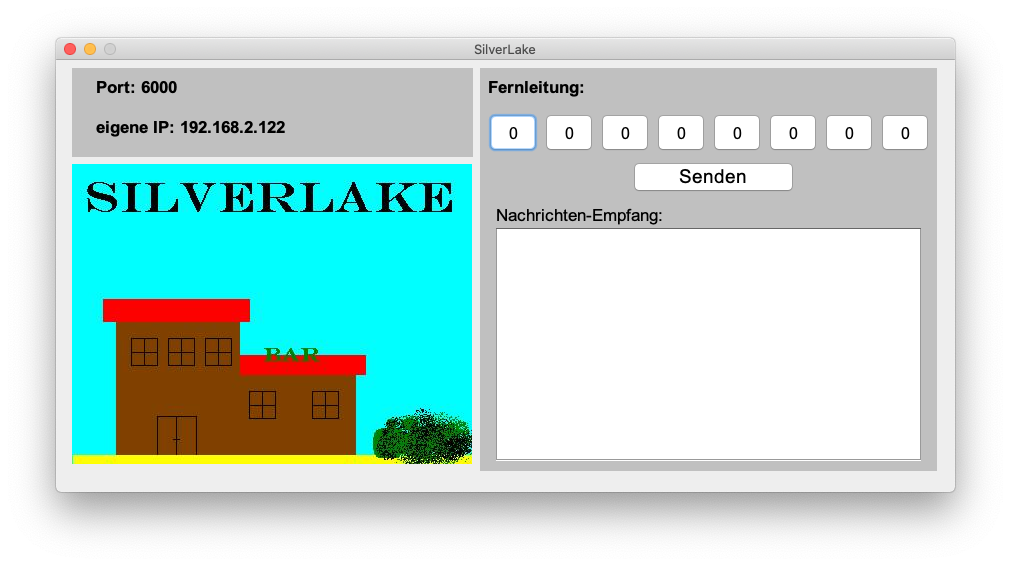
\includegraphics[width=.9\columnwidth]{Q2-GK-AB.II.2-Abb_Silver Lake.png}

	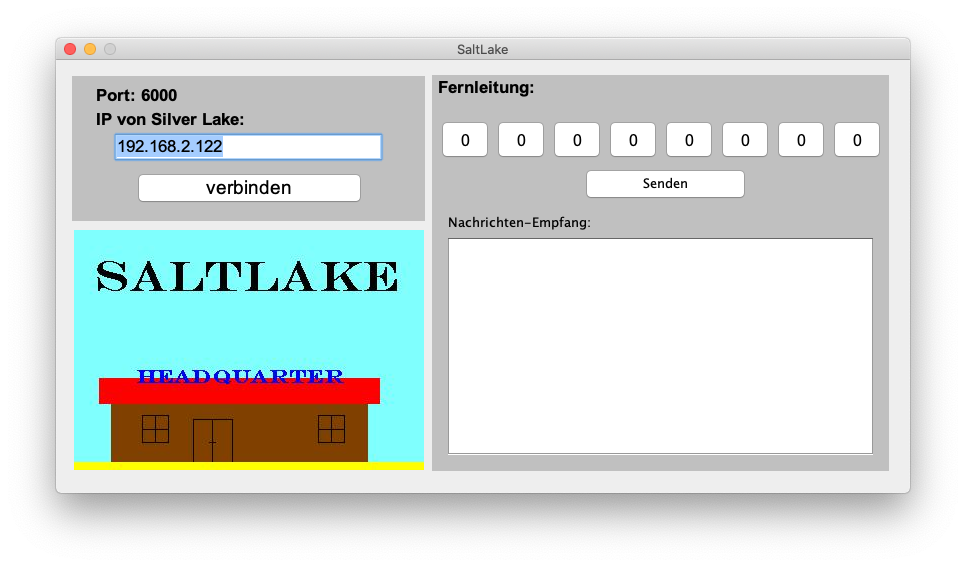
\includegraphics[width=.9\columnwidth]{Q2-GK-AB.II.2-Abb_Saltlake.png}
\end{multicols}

\begin{aufgabe}
	Arbeitet in denselben Zweiergruppen, wie in der letzten Stunde und schaut euch erneut eure Zeichencodierung an. Es können immer acht Bit pro Nachricht übermittelt werden (siehe Abbildungen oben). Passt eure Codierung so an, dass sie mit dieser Art der Datenübertragung nutzbar ist.
\end{aufgabe}

\begin{aufgabe}
	Einer von euch startet das Programm \programm{SilverLake}, der andere von euch startet an irgendeinem anderen Rechner das Programm \programm{SaltLake} aus dem Tauschverzeichnis. Kommuniziert miteinander. Teilt dem anderen zum Beispiel mit, was euer momentaner Lieblingsfilm ist oder auf welches Gericht ihr im Moment Appetit hättet.
	
	Setzt euch nach etwa 10 Minuten \enquote{Unterhaltung} wieder zusammen.
\end{aufgabe}

\begin{aufgabe}
Hat die Kommunikation einwandfrei funktioniert oder gab es Verständigungsschwierigkeiten? Lassen sich die Verständigungsschwierigkeiten auch auf technische Probleme zurückführen? Haltet eure Erkenntnisse in Stichpunkten fest.
\end{aufgabe}

Fehler bei der Datenübertragung können mit unterschiedlichen Prüfverfahren erkannt werden. Drei wichtige Verfahren sind die folgenden:
\begin{itemize}
	\item \emph{Paritätsbit}: Dem eigentlichen Datenblock wird ein sogenanntes \emph{Paritätsbit} angehängt. Sind im Datenblock eine gerade Anzahl von Einsen vorhanden, so wird eine Null angehängt, andernfalls eine Eins.
	\item \emph{Prüfsumme}: Zuerst wird die Quersumme des Datenblocks berechnet. Von dieser Summe wird dann der Rest modulo $n$ berechnet und dem eigentlichen Datenblock angehängt.
		
		Hinweis: Bei $n = 2$ entspricht dies dem Paritätsbit-Verfahren. Warum?
	\item \emph{gewichtete Prüfsumme}: Die einzelnen Bits des Datenblocks werden mit einer individuellen Gewichtung (z. B. mit der Wichtungsfolge $1,2,3,4,\dots,m$) in die Quersumme eingerechnet. Auch hier wird der Rest modulo $n$ an den Datenblock angehängt.
\end{itemize}

\begin{aufgabe}
Wende die drei Prüfverfahren jeweils auf die Zahlenfolgen an: 
\begin{tasks}(4)
	\task \code{11001}
	\task \code{11000}
	\task \code{10101}
	\task \code{00010}
\end{tasks}

Warum ist es bei den Prüfsummenverfahren sinnvoll, für $n$ eine Zweierpotenz zu wählen?
\end{aufgabe}

\begin{aufgabe}
Häufige Fehlerquellen sind: Kippen eines Bits und Vertauschen zweier Bits. Zeige jeweils an einem Beispiel, welches der drei Prüfverfahren den ersten bzw. zweiten Fehler erkennt bzw. nicht erkennt.
\end{aufgabe}

\begin{aufgabe}
	Welche der Sendungen sind wahrscheinlich fehlerfrei?
	
	\begin{tabularx}{\textwidth}{lXXXXX}
	Prüfbit: & a) \code{11001 1} & b) \code{10111 1} & c) \code{00000 0} & d) \code{11111 1} & e) \code{00101 1} \\
	Quersumme ($n=4$): & a) \code{11001 11} & b) \code{10111 01} & c) \code{00000 00} & d) \code{11111 01} & e) \code{00101 10} \\
	gew. Quers. ($n=4$): & a) \code{11001 00} & b) \code{10111 10} & c) \code{00000 10} & d) \code{11111 11} & e) \code{00101 00}
	\end{tabularx}
\end{aufgabe}

\end{document}
